\title{Lecture 11\\Problem Solvers of Intelligent Systems \vspace{-2em}}

\begin{frame}
	\titlepage
\end{frame}

\begin{frame}{\\Contents}
	\topline
	\justifying
	
	Models for solving problems in the absence of stored solution methods. Plausible reasoning. The knowledge processing engine of an intelligent system as a multi-agent system. The concept of a multi-agent system.
	
\end{frame}

\begin{frame}{Modern approaches to problem solving}
	\topline
	\justifying
	\vspace*{\fill}
	
	\footnotesize
	
	\vspace{2mm}
	\textbf{Solving Problems Using Stored Programs}
	
	\vspace{1mm}
	In this case, it is assumed that the system already has a program
	solutions to problems of a given class, and the solution comes down to finding such a program
	and its interpretation on the given input data. Towards systems oriented
	This approach includes, in particular:
	\begin{textitemize}
		\item programs written in programming languages such as imperative,
		as well as the declarative paradigm (including logical and functional);
		\item implementation of genetic algorithms;
		\item neural network models of information and knowledge processing.
	\end{textitemize}
	
	\vspace{1mm}
	It should be noted that even in the case of using a stored program the solution to the problem is not always trivial: firstly, it is necessary to find a suitable program based on the specification, secondly, to ensure its
	correct interpretation.
	
\end{frame}

\begin{frame}{Modern approaches to problem solving}
	\topline
	\justifying
	\vspace*{\fill}
	
	\footnotesize
	
	\vspace{2mm}
	\textbf{Solving problems in conditions where the solution program is unknown}
	
	\vspace{1mm}
	In this case, the system may not have a ready-made solution program for the class.
	tasks to which the formulated task relates. Therefore, they are used
	additional, relatively general methods for finding a solution, not
	designed for a narrow class of tasks, for example:
	\begin{textitemize}
		\item splitting a task into subtasks;
		\item methods for searching solutions in depth and breadth;
		\item random search method and trial and error method;
		\item bisection method and other heuristics.
	\end{textitemize}
	
	Various models of logical inference are also used:
	\begin{textitemize}
		\item deductive, inductive and abductive models;
		\item models based on fuzzy logic and default logic;
		\item models based on temporal logic and other variants of formal inference.
	\end{textitemize}
	
\end{frame}

\begin{frame}{Problem Solver}
	\topline
	\justifying
	
	\begin{SCn}
		\scnheader{cybernetic system problem solver}
		\scnidtf{a component of a cybernetic system responsible for solving specific problems using existing methods}
		\scntext{feature}{The main feature of problem solvers is the need to solve problems in conditions where the information needed for the solution is not explicitly localized and must be found during the solution process based on specified criteria and search strategies.}
	\end{SCn}
\end{frame}

\begin{frame}{Cybernetic System Problem Solver}
	\topline
	\justifying
	\vspace*{\fill}\\
	\begin{SCn}
		\scnheader{cybernetic system problem solver}
		\scnidtf{the totality of all skills and problem-solving methods possessed by a cybernetic system at a given moment in time}
		\scntext{explanation}{The modern approach to constructing problem solvers assumes their modifiability: a cybernetic system can acquire new \textit{skills} as needed, refine existing ones, and even abandon some skills to improve performance. Therefore, it makes sense to speak not of a rigidly fixed solver, defined once during the system's creation, but of a set of skills, fixed at each moment in time but constantly evolving.}
	\end{SCn}
\end{frame}

\begin{frame}{Types of Problem Solvers}
	\topline
	\justifying
	\vspace*{\fill}\\
	\begin{SCn}
		\scnheader{cybernetic system problem solver}
		\scnsuperset{united cybernetic system problem solver}
		\begin{scnindent}
			\scnidtf{complete cybernetic system problem solver}
			\scnidtf{integrated cybernetic system problem solver}
			\scnidtf{problem solver that implements all the system's functional capabilities, both primary and secondary}
		\end{scnindent}
		\scnsuperset{hybrid cybernetic system problem solver}
		\begin{scnindent}
			\scnidtf{problem solver that implements two or more problem-solving models}
		\end{scnindent}
	\end{SCn}
\end{frame}

\begin{frame}{United Problem Solver}
	\topline
	\justifying
	\vspace*{\fill}\\
	\small{
		\begin{SCn}
			\scnheader{united cybernetic system problem solver}
			\scntext{explanation}{In general, a united cybernetic system problem solver solves problems related to:
				\begin{textitemize}
					\item providing the basic functional capabilities of the system (for example, solving clearly formulated problems at the user’s request);
					\item ensuring the correctness and optimization of the operation of the cybernetic system itself throughout its entire life cycle;
					\item ensuring advanced training for end users and system developers (training and maintenance support);
					\item ensuring automation of development and management of the development of the cybernetic system itself.
			\end{textitemize}}
		\end{SCn}
	}
\end{frame}

\begin{frame}{Models for solving problems in the absence of stored solution methods}
	\topline
	\justifying
	
	\footnotesize
	\vspace{10mm}
	
	They are used in situations where the system does not have a ready-made solution to a problem, and the solution path has to be \uline{constructed}, \uline{searched for} or \uline{generated} directly in the process of work.
	
	Such situations include:
	\begin{textitemize}
		\item the problem is new and there is no pre-prepared solution method for it;
		\item the conditions of the problem are not fully specified, contain uncertainty or contradictions;
		\item the system has individual knowledge and rules, but does not have a ready-made plan for their application to a given task;
		\item the problem is too complex for direct enumeration and requires decomposition, heuristics, or plausible reasoning;
		\item solution must be obtained in a changing environment, where a stored method quickly loses its relevance.
	\end{textitemize}
\end{frame}

\begin{frame}{Problem Statement}
	\topline
	\justifying
	
	\begin{textitemize}
		\item For many problems, it is impossible to store in advance a ready-made solution program for every possible case.
		\item The state space may be too large, incomplete, probabilistic, or partially observable.
		\item Search, inference, heuristics, learning and adaptation models are used.
	\end{textitemize}
\end{frame}

\begin{frame}{Historical stages of AI}
	\topline
	\justifying
	
	\begin{textitemize}
		\item 1950s–1960s: Automatic problem solvers, theorem provers, heuristic search.
		\item 1969–1980s: Expert systems and rule-based reasoning.
		\item Since 1986: The return of neural networks thanks to backpropagation.
		\item Since the late 1980s: probabilistic models, machine learning,  deep learning.
	\end{textitemize}
\end{frame}

\begin{frame}{Early approaches}
	\topline
	\justifying
	
	\begin{textitemize}
		\item Some of the early directions were state-space search, automated theorem proving, and heuristic search control.
		\item During this period, General Problem Solver, Logic Theorist, and other systems oriented toward universal solution strategies emerged.
		\item The idea was not to store a ready-made answer, but to build a chain of steps towards the goal.
	\end{textitemize}
\end{frame}

\begin{frame}{General Problem Solving Strategies}
	\topline
	\justifying
	
	\begin{textitemize}
		\item splitting a task into subtasks;
		\item solution of the problem "from the end"{} (reverse inference);
		\item simplification of the task and transition to a more convenient description language;
		\item enumeration, random search and trial and error method;
		\item use of analogy, patterns and typical classes of problems.
	\end{textitemize}
\end{frame}

\begin{frame}{State space}
	\topline
	\justifying
	
	\footnotesize
	\vspace{10mm}
	
	A state space is a set of possible problem states, interconnected by admissible transitions. In such a model, solving a problem is interpreted as finding a path that takes the system from its initial state to its target state.
	
	\vspace{2mm}
	
	To define the state space, it is necessary to determine:
	\begin{textitemize}
		\item initial state of the task;
		\item target state or set of admissible target states;
		\item operations of transition from one state to another;
		\item restrictions on the admissibility of states and transitions.
	\end{textitemize}
	
	\vspace{2mm}
	
	Thus, the solution to the problem is reduced to constructing a sequence of admissible transitions leading from the initial state to one of the target states.
\end{frame}

\begin{frame}{AND-subgoals and OR-subgoals}
	\topline
	\justifying
	
	\footnotesize
	\vspace{10mm}
	
	When describing a solution process, a complex goal is often represented as a system of subgoals. These subgoals can be linked by \uline{AND} and \uline{OR} relationships, which allows for defining the structure of the solution search.
	
	\vspace{2mm}
	
	\begin{textitemize}
		\item \uline{AND-subgoals} mean that in order to achieve the overall goal, it is necessary to solve all related subtasks;
		\item \uline{OR-subgoals} mean that to achieve the goal it is sufficient to solve at least one of several alternative subgoals;
		\item The combination of AND and OR subgoals allows one to represent the solution to a problem in the form of a tree or a search graph.
	\end{textitemize}
	
	\vspace{2mm}
	
	For example, if the goal is to diagnose a technical malfunction, then several tests may be required to confirm one hypothesis, and there may be several alternative paths to choosing a method for eliminating the malfunction.
\end{frame}

\begin{frame}{Searching the state space}
	\topline
	\justifying
	
	\footnotesize
	\vspace{10mm}
	
	State space search involves the sequential generation, analysis, and selection of states that potentially lead to the goal. The order in which states are considered is determined by the chosen search strategy.
	
	\vspace{2mm}
	
	The most common search directions are:
	\begin{textitemize}
		\item \uline{depth-first} search, in which one selected branch of the solution is first developed;
		\item \uline{breadth-first} search, in which all states of the current level are considered sequentially;
		\item search \uline{from source data to target}, corresponding to the direct deployment of the solution process;
		\item search \uline{from the target to the source data}, corresponding to the inverse construction of the solution.
	\end{textitemize}
	
	\vspace{2mm}
	
	The choice of strategy depends on the structure of the state space, the number of possible transitions, the depth of the solution, and the available information about the problem.
\end{frame}

\begin{frame}{Splitting a task into subtasks}
	\topline
	\justifying
	
	\begin{textitemize}
		\item The original problem is divided into simpler subproblems, the solution of which is more accessible.
		\item Then the solutions of the subproblems are combined into a final solution.
		\item This approach is associated with hierarchical planning and the divide-and-conquer strategy.
	\end{textitemize}
\end{frame}

\begin{frame}{Reverse output}
	\topline
	\justifying
	
	\begin{textitemize}
		\item In backward inference, the system starts with a goal and looks for rules or statements that can justify it.
		\item Then each premise is turned into a subgoal.
		\item This approach has been widely used in logical and expert systems.
	\end{textitemize}
\end{frame}

\begin{frame}{Depth-first and breadth-first search}
	\topline
	\justifying
	
	\begin{textitemize}
		\item \textbf{Depth-first search} quickly goes down one branch, but can get stuck in a dead end.
		\item \textbf{Breadth-first search} is systematic and finds the shortest solution in the number of steps, but requires a lot of memory.
		\item These strategies formed the basis of many state-space problem solvers.
	\end{textitemize}
\end{frame}

\begin{frame}{Heuristic Search}
	\topline
	\justifying
	
	\begin{textitemize}
		\item Heuristics reduce search complexity by using domain knowledge.
		\item Instead of a complete enumeration, the system evaluates which states are more promising.
		\item A classic example is best-first search and A*-search (search by the first best match on a graph).
	\end{textitemize}
\end{frame}

\begin{frame}{Random search and enumeration}
	\topline
	\justifying
	
	\begin{textitemize}
		\item If the solution space is small or poorly structured, random search and trial and error can be used.
		\item A more systematic option is a complete enumeration with checking of variants and rollback.
		\item These methods are simple, but do not scale well.
	\end{textitemize}
\end{frame}

\begin{frame}{Analogy and Templates}
	\topline
	\justifying
	
	\begin{textitemize}
		\item In a number of cases, the problem is solved by comparing it with an already known type of problem.
		\item Analogy allows us to transfer the structure of a solution from one area to another.
		\item This is close to case-based reasoning and the use of precedents.
	\end{textitemize}
\end{frame}

\begin{frame}{Logical models of problem solving}
	\topline
	\justifying
	
	\begin{textitemize}
		\item Logical models represent knowledge in a formal form and allow one to draw conclusions about new facts.
		\item They are especially convenient where rigor, explainability, and control over the correctness of reasoning are important.
		\item In such models, the task often boils down to proving a goal from a set of facts and rules.
	\end{textitemize}
\end{frame}

\begin{frame}{Classification of logical reasoning}
	\topline
	\justifying
	
	\begin{textitemize}
		\item \textbf{Deduction:} derivation of the particular from the general.
		\item \textbf{Induction:} generalization based on a set of particular observations.
		\item \textbf{Abduction:} search for the most plausible explanation of an observed fact.
	\end{textitemize}
\end{frame}

\begin{frame}{Plausible reasoning}
	\topline
	\justifying
	
	\begin{textitemize}
		\item Plausible reasoning is used when there is insufficient information for rigorous proof.
		\item In this case, the system does not construct an absolutely guaranteed conclusion, but the most reasonable or probable one.
		\item These include \textit{abductive inference}, \textit{default inference}, \textit{fuzzy inference}, and \textit{probabilistic inference}.
	\end{textitemize}
\end{frame}

\begin{frame}{Logical Languages and Systems}
	\topline
	\justifying
	
	\begin{textitemize}
		\item \textbf{Prolog} is widely used for logic programming.
		\item For production systems, rule-based environments are used, for example \textbf{CLIPS}.
		\item These tools are used in expert systems, rule interpreters and automatic inference systems.
	\end{textitemize}
\end{frame}

\begin{frame}{Examples of logical and expert systems}
	\topline
	\justifying
	
	\vspace{10mm}
	
	\begin{textitemize}
		\item \textbf{DENDRAL} --- one of the first expert systems designed for chemical analysis and identification of the structure of organic compounds.
		\item \textbf{MYCIN} --- a medical consultation system that used production rules to diagnose bacterial infections and select therapy.
		\item \textbf{PROSPECTOR} --- expert system for geological exploration and assessment of the probability of the presence of minerals.
		\item \textbf{INTERNIST} --- a medical decision support system focused on the diagnosis of internal diseases.
		\item \textbf{R1 (XCON)} --- expert system for configuring computing systems according to specified requirements.
	\end{textitemize}
\end{frame}

\begin{frame}{Limitations of Purely Logical Models}
	\topline
	\justifying
	
	\begin{textitemize}
		\item A pure logical model requires labor-intensive manual description of knowledge.
		\item Rigid formalization does not work well in environments with uncertainty and variable data.
		\item Therefore, logical models are often combined with probabilistic, learning and heuristic approaches.
	\end{textitemize}
\end{frame}

\begin{frame}{Machine learning}
	\topline
	\justifying
	
	\begin{textitemize}
		\item Machine learning is used when it is not possible to explicitly program in advance a way to solve all situations.
		\item Instead of a ready-made algorithm, the system learns from data and experience.
		\item Basic modes: supervised, unsupervised, and reinforcement learning.
	\end{textitemize}
\end{frame}

\begin{frame}{Neural network models}
	\topline
	\justifying
	
	\begin{textitemize}
		\item Neural networks are particularly effective for recognizing images, speech, text, and complex nonlinear relationships.
		\item After 1986, the backpropagation method gave a powerful impetus to the development of the neural network approach.
		\item The current stage is associated with deep learning: CNN, RNN, Transformers and other architectures.
	\end{textitemize}
\end{frame}

\begin{frame}{Advantages of neural networks}
	\topline
	\justifying
	
	\begin{textitemize}
		\item They allow us to solve problems for which it is difficult to formulate a set of rules manually.
		\item The network itself extracts useful features from the data during the training process.
		\item However, neural network solutions are often less interpretable than logical models.
	\end{textitemize}
\end{frame}

\begin{frame}{Genetic Algorithms}
	\topline
	\justifying
	
	\vspace{10mm}
	\footnotesize
	
	\begin{columns}[T,totalwidth=\textwidth]
		\begin{column}{0.56\textwidth}
			
			\vspace{10mm}
			
			\begin{textitemize}
				\item Genetic algorithms model natural selection in solution space.
				\item Each possible solution is encoded as a set of parameters (genotype) and evaluated using a fitness function.
				\item The search process uses selection, crossover, and mutation operations, which allows for a gradual improvement in the quality of solutions.
				\item This approach is especially useful for complex nonlinear optimization and search problems.
			\end{textitemize}
		\end{column}
		
		\begin{column}{0.40\textwidth}
			\begin{center}
				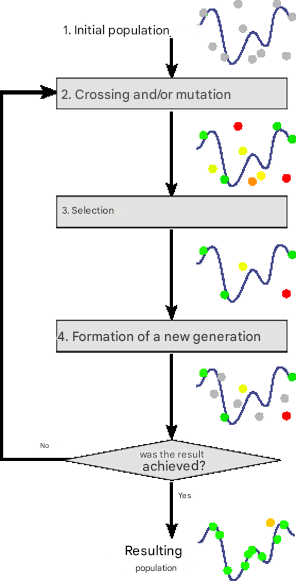
\includegraphics[width=0.8\linewidth]{part2/images/is_problem_solvers/gen_en.png}
			\end{center}
		\end{column}
	\end{columns}
\end{frame}

\begin{frame}{When Genetic Algorithms Are Useful}
	\topline
	\justifying
	
	\begin{textitemize}
		\item When the solution space is very large and there is no good analytical method.
		\item When it is necessary to search for an acceptable, and not necessarily strictly optimal, solution.
		\item When it is useful to explore many alternative options in parallel.
	\end{textitemize}
\end{frame}

\begin{frame}{Hybrid Models}
	\topline
	\justifying
	
	\begin{textitemize}
		\item In practice, hybrid systems are increasingly used: logic + probabilities, rules + learning, neural networks + evolutionary methods.
		\item Genetic algorithms can be used to tune neural networks, and logical rules can be used to interpret ML results.
		\item The hybrid approach allows for the combination of explainability, flexibility, and adaptability.
	\end{textitemize}
\end{frame}

\begin{frame}{Comparison of approaches}
	\topline
	\justifying
	
	\begin{textitemize}
		\item \textbf{Search and heuristics} are good for explicit state spaces.
		\item \textbf{Logical models} are strong in explainable inference and formal correctness.
		\item \textbf{Machine learning and neural networks} are effective on big data and complex dependencies.
		\item \textbf{Genetic algorithms} are useful for global search and optimization.
	\end{textitemize}
\end{frame}

\begin{frame}{Conclusion: Models for solving problems in the absence of stored methods for their solution}
	\topline
	\justifying
	
	In the absence of a stored solution method, the problem is solved not by extracting a ready-made program, but by constructing a solution path based on search, logical inference, heuristics, plausible reasoning, learning, and adaptation.
	
	\bigskip
	
	The history of AI shows that the most powerful systems emerge when these approaches are not opposed but \uline{combined}.
\end{frame}

\begin{frame}{Decentralized Artificial Intelligence (DAI)}
	\topline
	\justifying
	\begin{textitemize}
		\item The multi-agent approach considers a complex system as a community of autonomous participants operating in a common environment --- a multi-agent system (MAS)
		\item This view is especially useful where knowledge, resources, and decisions are distributed across many nodes
	\end{textitemize}
\end{frame}

\begin{frame}{Why MAS are important today}
	\topline
	\justifying
	\begin{textitemize}
		\item Modern digital systems are rarely fully centralized: they combine autonomy, messaging, and coordination.
		\item The multi-agent model helps design robust, scalable, and flexible solutions under uncertainty.
		\item With the development of LLM, interest in MAS has increased as complex tasks are increasingly decomposed into interacting roles and functions.
	\end{textitemize}
\end{frame}

\begin{frame}{What is a multi-agent system}
	\topline
	\justifying
	\begin{textitemize}
		\item A multi-agent system is a set of interacting agents operating in a common environment and solving problems in a distributed manner.
		\item The global behavior of the MAS arises from the local actions of agents, their exchange of messages, cooperation, competition, and coordination.
		\item Key idea: knowledge, goals and resources are distributed, so there is no need for a single, fully informed center.
	\end{textitemize}
\end{frame}

\begin{frame}{Agent as a cybernetic system}
	\topline
	\justifying
	\begin{textitemize}
		\item From a cybernetics perspective, an agent is a control system that has a boundary, inputs, outputs, state, goals, and feedback loops.
		\item An agent perceives the environment, interprets signals, makes decisions, and influences the environment through actions
		\begin{textitemize}
			\item Interaction with the environment (sensors, effectors)
			\item Interaction with other agents
			\item Decision Making
		\end{textitemize}
	\end{textitemize}
\end{frame}

\begin{frame}{Key properties of the agent}
	\topline
	\justifying
	\begin{textitemize}
		\item Autonomy: the agent itself chooses actions within the framework of its architecture and goals.
		\item Reactivity: the agent responds to changes in the environment; proactivity: it initiates actions itself.
		\item Sociality: The agent is able to interact with other agents through messages, protocols, and shared rules.
		\item Additionally, learning ability, adaptability, mobility and rationality are highlighted.
	\end{textitemize}
\end{frame}

\begin{frame}{MAS Environment}
	\topline
	\justifying
	\begin{textitemize}
		\item Environment is the space of states, objects, resources, and events in which agents observe and act.
		\item The environment sets constraints: observability, resource availability, time dynamics, level of uncertainty, and permissible actions.
		\item In modern engineering, the environment is often implemented as a digital infrastructure: software interfaces, databases, message brokers, sensors, simulators.
	\end{textitemize}
\end{frame}

\begin{frame}{The "agent---environment---other agents"{}\\ model}
	\topline
	\justifying
	\begin{textitemize}
		\item Each agent has a local model of the world, which is usually incomplete and may differ from the models of other agents.
		\item Coordination occurs through the exchange of messages, through the\\ environment, or through organizational rules.
		\item From here follow the typical tasks of the MAS: coordination, distribution of roles, conflict resolution and achieving a collective effect.
	\end{textitemize}
\end{frame}

\begin{frame}{Agent Interaction Language}
	\topline
	\justifying
	\begin{textitemize}
		\item The agent interaction language describes the form, meaning, and pragmatics of messages between agents.
		\item It specifies the communication types of messages, such as request, inform, propose, agree, refuse; the structure of the content and sometimes the ontology of the subject domain.
		\item Such a language is needed not only for syntax, but also for interpreting intentions and coordinating distributed behavior.
	\end{textitemize}
\end{frame}

\begin{frame}{MAS Features}
	\topline
	\justifying
	\begin{textitemize}
		\item Decentralization: the solution does not come down to a single computing node or a single governance algorithm.
		\item Heterogeneity: agents can have different goals, knowledge, architectures and levels of rationality.
		\item Locality and distribution: each agent works with partial information and limited resources.
		\item Emergence: the collective behavior of a system can be richer than the behavior of individual participants.
	\end{textitemize}
\end{frame}

\begin{frame}{Advantages of MAS}
	\topline
	\justifying
	\begin{textitemize}
		\item Scalability: It is easier to increase the number of agents than to build one super-complex central module.
		\item Fault tolerance: the failure of one agent does not always destroy the entire system.
		\item Flexibility: new agents, roles, and services can be added without completely redesigning the architecture.
		\item Naturalness of modeling: MAS describe logistics, markets, robots, energy grids, smart cities, and organizational processes well.
	\end{textitemize}
\end{frame}

\begin{frame}{Limitations and Complexities}
	\topline
	\justifying
	\begin{textitemize}
		\item It is difficult to ensure consistency of knowledge and predictability of global behavior.
		\item Communication and coordination create overhead in terms of time, network, and computation.
		\item Problems of trust, strategic behavior, deadlocks, races and conflicts for resources arise.
		\item Designing a MAS requires a combination of algorithms, organizational theory, communication protocols, and software engineering.
	\end{textitemize}
\end{frame}

\begin{frame}{Origins of the MAS Theory}
	\topline
	\justifying
	\begin{textitemize}
		\item The background of the MAS is connected with cybernetics, systems theory, research on self-organization and distributed control.
		\item Important precursors included the actor model, research on distributed AI, the bulletin board principle{}, and work on collective behavior.
		\item The development of the theory led to a transition from the description of individual agents to the consideration of organizational forms of collective intelligence.
	\end{textitemize}
\end{frame}

\begin{frame}{Timeline of Development}
	\topline
	\justifying
	\begin{textitemize}
		\item 1970s: actor model and the "blackboard" principle{}, ideas of distributed problem solving.
		\item 1980s: Distributed AI, cooperative problem solving, DVMT (Distributed Vehicle Monitoring Testbed), contract network, engineering coordination models.
		\item 1990s: formation of MAS theory, BDI architecture, ACL/KQML, FIPA, specialized platforms.
		\item 2000s--2020s: service and web agents, the Internet of Things, swarms, digital twins, and then LLM agents and agent AI.
	\end{textitemize}
\end{frame}

\begin{frame}{Key Milestones}
	\topline
	\justifying
	\begin{textitemize}
		\item actor model is associated with the work of Carl Hewitt; it showed how independent entities can interact through messages.
		\item blackboard systems like HEARSAY-II have become an important model for collaborative problem solving by several specialized components.
		\item Smith's contract network protocol has become a classic mechanism for distributing tasks through announcement, requests, and selection of a performer.
		\item The BDI approach described the agent in terms of beliefs, desires, and intentions.
	\end{textitemize}
\end{frame}

\begin{frame}{MAS Classification: General Logic}
	\topline
	\justifying
	\begin{textitemize}
		\item MAS are classified by architecture, type of environment, nature of goals, interaction mechanism, mobility and organizational form.
		\item The same project can be classified into several classes at once, so classifications are usually multi-criteria.
		\item This is important for the selection of coordination algorithms, communication languages and implementation tools.
	\end{textitemize}
\end{frame}

\begin{frame}{By the nature of the agents' goals}
	\topline
	\justifying
	\begin{textitemize}
		\item Cooperative systems: agents work towards a common goal and are usually willing to share information.
		\item Competitive or egoistic systems: agents have different interests, so mechanisms of bargaining, auctions and incentives are needed.
		\item Mixed systems: local interests are combined with system-wide constraints; this is typical for markets and platforms.
	\end{textitemize}
\end{frame}

\begin{frame}{By environment design}
	\topline
	\justifying
	\begin{textitemize}
		\item Fully and partially observable environment.
		\item Deterministic and stochastic; static and dynamic; discrete and continuous.
		\item An open environment allows agents to enter and exit; a closed environment assumes a fixed composition of participants.
	\end{textitemize}
\end{frame}

\begin{frame}{On the architecture of agents}
	\topline
	\justifying
	\begin{textitemize}
		\item Reactive agents rely on simple "situation-action"{} rules and respond quickly to the environment.
		\item Intelligent agents build internal models, plans and forecasts.
		\item Hybrid architectures combine a reactive layer with planning and coordination layers
	\end{textitemize}
\end{frame}

\begin{frame}{Hierarchical and non-hierarchical MAS}
	\topline
	\justifying
	\begin{textitemize}
		\item Hierarchical MAS are built around levels of management, delegation, and subordination; they are useful for control, monitoring, and task decomposition.
		\item Non-hierarchical MAS are based on peer agents, network exchange, and local rules; they better support flexibility and self-organization.
		\item In practice, hybrids are often used: the strategic level is hierarchical, and local interaction is carried out in a decentralized manner.
	\end{textitemize}
\end{frame}

\begin{frame}{Centralized, decentralized, hybrid}
	\topline
	\justifying
	\begin{textitemize}
		\item In a centralized scheme, a single coordinating agent or service makes key decisions.
		\item In a decentralized system, control is distributed and order arises through protocols and local rules.
		\item A hybrid scheme uses central logging, monitoring, or policy services, but retains the autonomy of the performers.
	\end{textitemize}
\end{frame}

\begin{frame}{On mobility and implementation}
	\topline
	\justifying
	\begin{textitemize}
		\item Software agents operate in networks, information systems, and web services.
		\item Mobile agents can move computation closer to data or services.
		\item Robotic agents are physically embodied and operate through sensors and actuators.
		\item In cyber-physical systems, the MAS connects digital and physical participants in a single control loop.
	\end{textitemize}
\end{frame}

\begin{frame}{Classification of agent interactions}
	\topline
	\justifying
	\begin{textitemize}
		\item Interactions are divided into cooperation, coordination, competition,\\ negotiations, coalitions and knowledge exchange.
		\item According to the channel, a distinction is made between direct communication, interaction through a environment, and mixed schemes.
		\item According to the duration of the connection, there are episodic contacts, stable roles and long-term organizational relationships.
	\end{textitemize}
\end{frame}

\begin{frame}{Coordination mechanisms: an overview}
	\topline
	\justifying
	\begin{textitemize}
		\item Coordination of actions in time, by resources, by roles, and by common constraints.
		\item Basic mechanisms: plans, rules, contracts, auctions, a common blackboard, organizational norms, and market signals.
		\item The choice of mechanism depends on the number of agents, the degree of conflict of interests and the variability of the environment.
	\end{textitemize}
\end{frame}

\begin{frame}{Task Planning and Allocation}
	\topline
	\justifying
	\begin{textitemize}
		\item Centralized distribution is convenient when observability is good, but it scales poorly.
		\item Distributed scheduling allows agents to independently propose and accept subtasks.
		\item Classic examples: task allocation, distributed problem solving, team planning, and collaborative planning.
	\end{textitemize}
\end{frame}

\begin{frame}{Contractual network and auction mechanisms}
	\topline
	\justifying
	\begin{textitemize}
		\item contract network protocol: a manager announces a task, potential performers submit bids, then a contractor is selected.
		\item Auction mechanisms are convenient when resources are limited and you need to quickly compare options.
		\item In modern systems, this class of ideas lives in logistics, cloud computing, robotics, and electronic markets.
	\end{textitemize}
\end{frame}

\begin{frame}{Coordination through a common environment}
	\topline
	\justifying
	\begin{textitemize}
		\item Environmental coordination means that agents interact indirectly, but through a shared context, blackboard, or action traces.
		\item A change in the environment serves as a signal to other participants.
		\item This approach is especially strong in swarm and weakly centralized systems.
	\end{textitemize}
\end{frame}

\begin{frame}{Organizational Coordination}
	\topline
	\justifying
	\begin{textitemize}
		\item The organizational approach defines roles, norms, powers, sanctions, and delegation procedures.
		\item Then coordination is ensured not only by messages, but also by the institutional structure of the system.
		\item It is precisely this transition from a “set of agents” to an “intelligent organization” that is important for modern organizational models.
	\end{textitemize}
\end{frame}

\begin{frame}{Languages and Standards:\\ KQML and FIPA ACL}
	\topline
	\justifying
	\begin{textitemize}
		\item KQML became one of the first widely used languages for exchanging messages between agents
		\item FIPA ACL took the idea of standardized communication further by adding a formal infrastructure, agent platform management, and interaction protocols.
		\item For interoperability, not only messages are important, but also vocabularies, ontologies, transport layer, and registration services.
	\end{textitemize}
\end{frame}

\begin{frame}{Performatives and Interactive Acts}
	\topline
	\justifying
	\begin{textitemize}
		\item Many ACLs are based on ideas from speech act theory: a message is viewed as an action with an intention.
		\item Performatives specify the type of intention: inform, request, query, propose, agree, refuse, confirm.
		\item This allows us to separate the content of the message from its communicative function.
	\end{textitemize}
\end{frame}

\begin{frame}{Ontologies, semantics, interoperability}
	\topline
	\justifying
	\begin{textitemize}
		\item Even a common ACL does not guarantee understanding without a common subject ontology and agreed-upon concepts.
		\item Therefore, in the MAS, term dictionaries, data schemas, content formats and interpretation rules are important
	\end{textitemize}
\end{frame}

\begin{frame}{Classic MAS platforms}
	\topline
	\justifying
	\begin{textitemize}
		\item Classic environments --- AgentBuilder, Grasshopper, Concordia, DESIRE, ADE, Telescript.
		\item JADE as a FIPA-compliant Java framework, Jason as a BDI platform, and SPADE as an XMPP/Python-oriented approach played a major role.
		\item These systems provided engineering templates: agent lifecycle, service catalogs, negotiation protocols, and debugging tools.
	\end{textitemize}
\end{frame}

\begin{frame}{Modern approaches to the development of MAS}
	\topline
	\justifying
	\begin{textitemize}
		\item Today, MAS are being developed as distributed event-driven systems: microservices, queues, software interfaces, digital twins, and simulations.
		\item Python, Java, Scala, Erlang/Elixir, Go are often used; AnyLogic, Mesa, NetLogo, Repast, GAMA are used for modeling.
		\item In industry, agent-based ideas are being combined with cloud architecture, stream processing, and reinforcement learning.
	\end{textitemize}
\end{frame}

\begin{frame}{Frames, languages, libraries}
	\topline
	\justifying
	\begin{textitemize}
		\item Classic: JADE, Jason, SPADE, Jadex, MadKit, Cougaar.
		\item For modeling and research: Mesa, Repast, NetLogo, GAMA; for robots --- ROS multi-agent add-ons.
		\item For LLM agents: AutoGen, CrewAI, LangGraph, OpenAI Agents SDK, Google ADK and related orchestrators.
	\end{textitemize}
\end{frame}

\begin{frame}{JADE, Jason, SPADE: A Brief Comparison}
	\topline
	\justifying
	\begin{textitemize}
		\item JADE is strong in FIPA compliance, service catalogs, containers, and distributed agent engineering in Java.
		\item Jason is useful for BDI programming and AgentSpeak when it is important to explicitly state beliefs, goals, and plans.
		\item SPADE is popular in the Python environment and plays well with network services and modern data libraries.
	\end{textitemize}
\end{frame}

\begin{frame}{Agent-oriented programming}
	\topline
	\justifying
	\begin{textitemize}
		\item In agent-oriented programming, the key entities are goals, intentions, roles, and protocols, not just classes and functions.
		\item An example of a specialized language is AgentSpeak; more generally, declarative rules and schedulers are used
		\item This style is especially useful where behavior must depend on the state of the environment and social context.
	\end{textitemize}
\end{frame}

\begin{frame}{Where are MAS used today}
	\topline
	\justifying
	\begin{textitemize}
		\item Logistics and transport, resource distribution, smart grids, production management.
		\item Swarm robots, market and city simulation, telecom, cyber-physical systems, digital platforms.
		\item In AI applications, MAS are used as a way to decompose a complex task into roles: planner, executor, critic, dispatcher, observer.
	\end{textitemize}
\end{frame}

\begin{frame}{LLM agents and classical MAS}
	\topline
	\justifying
	\begin{textitemize}
		\item An LLM agent is an agent in which a large language model plays a central role in perception, interpretation, or planning.
		\item LLM-MAS --- a special case of MAS, where some or all agents use LLM as a cognitive core.
		\item Therefore, not every multi-agent system contains LLM, but a system of several LLM agents already forms a modern variety of MAS.
	\end{textitemize}
\end{frame}

\begin{frame}{How do LLM agents differ from regular MAS?}
	\topline
	\justifying
	\begin{textitemize}
		\item Classical MAS is often built on explicitly defined rules, protocols, and domain models.
		\item LLM agents perform better with unstructured text, ambiguous tasks, and linguistic reasoning, but are less predictable.
		\item For them, prompt engineering, context, tools, memory, constraints, and fact checking are critical.
	\end{textitemize}
\end{frame}

\begin{frame}{New protocols and stack in agent-based AI}
	\topline
	\justifying
	\begin{textitemize}
		\item A new stack is formed around LLM agents: tool invocation, structured output, memory, MCP, A2A, and graph orchestrators.
		\item Unlike classic ACLs, what is important here is integration with external tools, knowledge search, and execution of actions in the digital environment.
		\item But the fundamental challenge remains the same: how to coordinate autonomous participants and achieve a reliable collective outcome.
	\end{textitemize}
\end{frame}

\begin{frame}{AutoGen, CrewAI, LangGraph, etc.}
	\topline
	\justifying
	\begin{textitemize}
		\item AutoGen develops conversational collaboration between agents; CrewAI emphasizes roles and workflows/teams.
		\item LangGraph constructs agent processes as a graph of states and transitions, which improves the manageability of complex scenarios.
		\item These tools are closer to orchestration tools than to classic MAS platforms, but the logic of distributed roles in them is the same.
	\end{textitemize}
\end{frame}

\begin{frame}{Architectural Shift: From MAS to New Types of Agent Systems}
	\topline
	\justifying
	\begin{textitemize}
		\item Previously, the main question was "how to design a collective of autonomous software entities?"
		\item Now the question is added: "how to integrate linguistic reasoning, tools and memory into the workflow of actions?"
		\item Therefore, modern agent systems of a new type combine the ideas of MAS, knowledge-based systems and LLM engineering.
	\end{textitemize}
\end{frame}

\begin{frame}{Practical implications for development}
	\topline
	\justifying
	\begin{textitemize}
		\item If the environment is well formalized, classic MAS models are useful: roles, protocols, auctions, BDI, and strong messages.
		\item If the task is textual, exploratory, or weakly structured, LLM agents with strong constraints and verification are effective.
		\item The most promising hybrid is: classical coordination plus LLM as a module for understanding, planning and explanation.
	\end{textitemize}
\end{frame}

\begin{frame}{Conclusion on the MAS}
	\topline
	\justifying
	\begin{textitemize}
		\item Multi-agent systems are a common model for describing distributed intelligence, coordination, and organizational behavior.
		\item Classical MAS provided the concepts of agency, protocols, and cooperation; modern LLM agents have extended this class of problems to include linguistic and instrumental interaction.
		\item Therefore, the topic of MAS remains key for AI, robotics, organization modeling and agentic software.
	\end{textitemize}
\end{frame}
